% !TEX program = xelatex
% Example deck for the tealnav theme, in Chinese: every layout the theme provides, plus a
% tips section with common presentation techniques (see references/beamer.md, Techniques).
% Needs XeLaTeX or Tectonic: xeCJKfntef and the TikZ spy library fail with ctex under LuaLaTeX.
% Build next to beamerthemetealnav.sty and logo.png: python3 <skill-dir>/scripts/slides.py build example.tex
\documentclass[aspectratio=169,11pt,fontset=fandol]{ctexbeamer}
\usetheme{tealnav}
\usepackage{booktabs}
\usepackage{pgfplots}
\pgfplotsset{compat=1.17}
\usetikzlibrary{positioning,arrows.meta,tikzmark,spy,overlay-beamer-styles}
% Packages used by the tips section.
\usepackage{xeCJKfntef}               % Chinese emphasis marks: \CJKunderdot, \CJKunderwave
\usepackage{tabularray}               % key-value tables with per-row and per-cell styles
\UseTblrLibrary{booktabs,siunitx}     % booktabs rules and decimal-aligned columns
\sisetup{mode=text}                   % numbers in the text font, matching the slide
\usepackage{qrcode}                   % QR codes drawn by TeX, no image files
\usepackage{fontawesome5,academicons} % general and academic-profile icons
\tcbuselibrary{raster}                % rows of equal-height tcolorbox cards

% Styles that take parameters must be defined outside frames.
\tikzset{
  stepbox/.style={draw=tealnavDark,rounded corners=2pt,minimum width=2.2cm,minimum height=0.9cm,
    align=center,alt=#1{fill=tealnavPeach,very thick}{fill=tealnavBlue}},
  steparrow/.style={-{Latex[length=2mm]},thick,tealnavDark},
}

% One line at the bottom of each tips frame naming the commands used.
\newcommand{\tip}[1]{\par\vfill
  {\raggedright\footnotesize\color{tealnavDark!65}\faLightbulb[regular]\enspace #1\par}}

\title{用 \LaTeX{} Beamer 制作学术报告}
\subtitle{tealnav 主题示例}
\author{示例作者}
\institute{示例单位}
\date{2026 年 10 月 7 日}
\titlegraphic{
\includegraphics[height=1cm]{logo}} % logo.png sits next to this file

\begin{document}

\begin{frame}[plain]
  \titlepage
\end{frame}

\begin{frame}[plain]
  \tableofcontents
\end{frame}

% \sectionaside{...} appears only on the outline; the optional short title feeds the top bar.
\section{引入\sectionaside{Introduction}}

\begin{frame}{为什么用 Beamer 做报告}
  \textbf{一句话}：用\alert{代码}写幻灯片，编译得到 PDF。

  \medskip
  \begin{itemize}
    \item 主题统一控制颜色、字体和版式，内容与样式分离
    \item 公式、代码、参考文献和论文共用同一套工具链
    \item 纯文本源文件，便于版本管理和协作修改
  \end{itemize}
\end{frame}

\section[基本元素]{基本元素\sectionaside{Basic Elements}}

\begin{frame}{列表、编号与强调}
  \begin{columns}[T]
    \column{0.46\textwidth}
    \textbf{无序列表}
    \begin{itemize}
      \item 每条只写一个要点
      \item 关键词用 \alert{\textbackslash alert} 强调
      \item 第二层列表
      \begin{itemize}
        \item 层级不宜超过两层
      \end{itemize}
    \end{itemize}
    \column{0.46\textwidth}
    \textbf{编号列表}
    \begin{enumerate}
      \item 先讲问题
      \item 再讲方法
      \item 最后给证据
    \end{enumerate}
  \end{columns}
\end{frame}

\begin{frame}{提示框}
  \begin{block}{普通提示}
    结论、定义或需要观众记住的一句话。
  \end{block}
  \begin{alertblock}{注意事项}
    醒目的警告；框内列表会跟随提示色：
    \begin{itemize}
      \item 编译失败时先看第一条错误
      \item 溢出时先删减内容，再调整版式
    \end{itemize}
  \end{alertblock}
\end{frame}

\section[图表公式]{图表与公式\sectionaside{Figures, Tables and Math}}

\begin{frame}{图文并排：左侧结论，右侧证据}
  \begin{columns}[c]
    \column{0.42\textwidth}
    \begin{itemize}
      \item 方法 B 在训练后期\alert{持续领先}
      \item 两条曲线在第 4 轮后拉开差距
      \item 数据为示意，非真实实验
    \end{itemize}
    \column{0.54\textwidth}
    \centering
    \begin{tikzpicture}
      \begin{axis}[width=\linewidth,height=0.62\textheight,
          xlabel={训练轮数},ylabel={准确率 (\%)},
          legend pos=south east,legend style={font=\scriptsize,draw=none,fill=none},
          tick label style={font=\scriptsize},label style={font=\small},
          axis lines=left,ymin=50,ymax=95]
        \addplot[mark=*,mark size=1.5pt,color=tealnavDark] coordinates
          {(1,58) (2,66) (3,71) (4,74) (5,76) (6,77) (7,78)};
        \addplot[mark=square*,mark size=1.5pt,color=tealnavOrange] coordinates
          {(1,57) (2,67) (3,74) (4,80) (5,84) (6,86) (7,88)};
        \legend{方法 A,方法 B}
      \end{axis}
    \end{tikzpicture}
  \end{columns}
\end{frame}

\begin{frame}{表格：只保留支撑结论的行和列}
  \centering
  \begin{tabular}{lccc}
    \toprule
    方法 & 准确率 (\%) & 参数量 & 推理时间 (ms) \\
    \midrule
    基线 A & 76.4 & 110M & 12.1 \\
    基线 B & 78.9 & 340M & 31.5 \\
    本文方法 & \textbf{\alert{84.2}} & 120M & 13.0 \\
    \bottomrule
  \end{tabular}

  \bigskip
  {\small 粗体为最好结果；数据为示意。}
\end{frame}

\begin{frame}{公式：先给直觉，再给定义}
  最小二乘回归要找一组参数，让预测值与观测值的平方误差最小：
  \[
    \hat{\boldsymbol\beta} = \arg\min_{\boldsymbol\beta}\;
      \bigl\lVert \mathbf{y} - X\boldsymbol\beta \bigr\rVert_2^2
    = \bigl(X^\top X\bigr)^{-1} X^\top \mathbf{y}.
  \]
  \begin{itemize}
    \item $X$：$n\times d$ 的设计矩阵；$\mathbf{y}$：$n$ 维观测向量
    \item 闭式解要求 $X^\top X$ 可逆\footnote{不可逆时可加入正则项，即岭回归。}
  \end{itemize}
\end{frame}

\section[代码绘图]{代码与绘图\sectionaside{Code and TikZ}}

\begin{frame}[fragile]{代码与效果：上下排列}
  \begin{codeexample}
\begin{tabular}{lc}
  \toprule
  Item & Quantity \\
  \midrule
  Apples & 3 \\
  \bottomrule
\end{tabular}
  \end{codeexample}
\end{frame}

\begin{frame}[fragile]{代码与效果：左右并排}
  \begin{codeside}
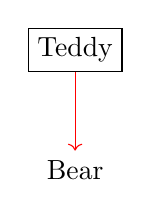
\begin{tikzpicture}
  \node (a) [draw] {Teddy};
  \node (b) [below=of a] {Bear};
  \draw[->, red] (a) -- (b);
\end{tikzpicture}
  \end{codeside}
\end{frame}

\begin{frame}{TikZ 流程图}
  \centering
  \begin{tikzpicture}[node distance=1.1cm,
      box/.style={draw=tealnavDark,fill=tealnavBlue,rounded corners=2pt,
        minimum width=2.3cm,minimum height=0.9cm,align=center},
      arrow/.style={-{Latex[length=2mm]},thick,tealnavDark}]
    \node[box] (src) {阅读材料};
    \node[box,right=of src] (plan) {规划大纲};
    \node[box,right=of plan] (write) {编写页面};
    \node[box,right=of write,fill=tealnavPeach] (check) {编译检查};
    \draw[arrow] (src) -- (plan);
    \draw[arrow] (plan) -- (write);
    \draw[arrow] (write) -- (check);
    \draw[arrow] (check.south) -- ++(0,-0.6) -| node[pos=0.25,below,font=\small]{渲染看图后修改} (write.south);
  \end{tikzpicture}
\end{frame}


\section[实用技巧]{实用技巧\sectionaside{Tips and Tricks}}

\begin{frame}{逐条讲解：未讲到的要点半透明}
  \setbeamercovered{transparent=15}
  \begin{itemize}[<+-| alert@+>]
    \item 观众先看到整页结构，知道接下来要讲几点
    \item 正在讲的一条自动换成强调色
    \item 讲过的条目恢复正常颜色，留在页面上便于回顾
  \end{itemize}
  \tip{\texttt{\textbackslash setbeamercovered\{transparent\}} 与 \texttt{[<+-| alert@+>]}；每步一页，PDF 翻页即动画}
\end{frame}

\begin{frame}{文字强调的几种方式}
  \begin{itemize}
    \item 颜色强调：\alert{关键结论}，适合一页里唯一的重点
    \item 加粗：\textbf{术语首次出现}，中文没有斜体，不要用 \texttt{\textbackslash emph}
    \item 着重号：\CJKunderdot{逐字强调}；波浪线：\CJKunderwave{存疑之处}
    \item 底色标记：\colorbox{tealnavPeach}{数字或短语}，像荧光笔
    \item 删除线：\CJKsout{旧说法}，配合新说法做对比
  \end{itemize}
  \tip{\texttt{xeCJKfntef} 提供中文着重号、波浪线和删除线（需 XeLaTeX）}
\end{frame}

\begin{frame}{公式分项标注}
  \vspace{1.2em}
  \[
    \tikzmarknode[fill=tealnavBlue,rounded corners=2pt,inner sep=2pt]{lhs}{\hat{\boldsymbol\beta}}
    = \arg\min_{\boldsymbol\beta}\;
    \tikzmarknode[fill=tealnavPeach,rounded corners=2pt,inner sep=2pt]{fit}
      {\bigl\lVert \mathbf{y} - X\boldsymbol\beta \bigr\rVert_2^2}
    + \tikzmarknode[fill=tealnavLavender,rounded corners=2pt,inner sep=2pt]{reg}
      {\lambda \lVert \boldsymbol\beta \rVert_2^2}
  \]
  \begin{tikzpicture}[remember picture,overlay,
      note/.style={font=\small,align=center,text=tealnavDark},
      pin/.style={-{Latex[length=1.6mm]},thick,tealnavDark!70}]
    \draw[pin,visible on=<2->] (fit.south) -- ++(0,-0.7) node[note,below] {拟合误差：\\预测与观测的差距};
    \draw[pin,visible on=<3->] (reg.north) -- ++(0,0.6) node[note,above] {正则项：限制参数大小};
    \draw[pin,visible on=<4->] (lhs.south) -- ++(0,-0.7) node[note,below] {岭回归估计};
  \end{tikzpicture}
  \vspace{4.5em}
  \tip{\texttt{\textbackslash tikzmarknode} 给公式片段命名并上色，再用 \texttt{remember picture} 画标注；\texttt{visible on=<2->} 控制出现顺序}
\end{frame}

\begin{frame}{流程图逐步出现，版面不跳动}
  \centering
  \begin{tikzpicture}[node distance=0.9cm]
    \node[stepbox=<1>] (a) {收集数据};
    \node[stepbox=<2>,right=of a,visible on=<2->] (b) {训练模型};
    \node[stepbox=<3>,right=of b,visible on=<3->] (c) {评估结果};
    \node[stepbox=<4>,right=of c,visible on=<4->] (d) {撰写报告};
    \draw[steparrow,visible on=<2->] (a) -- (b);
    \draw[steparrow,visible on=<3->] (b) -- (c);
    \draw[steparrow,visible on=<4->] (c) -- (d);
  \end{tikzpicture}

  \bigskip
  \only<1>{第一步：数据从哪里来}%
  \only<2>{第二步：模型怎么训练}%
  \only<3>{第三步：用什么指标评估}%
  \only<4>{第四步：结论怎么表述}
  \tip{TikZ 库 \texttt{overlay-beamer-styles}：\texttt{visible on=<2->} 预留位置后再显示，\texttt{alt=<2>\{…\}\{…\}} 让当前一步变色；带参数的样式要在导言区用 \texttt{\textbackslash tikzset} 定义}
\end{frame}

\begin{frame}{同一位置切换两张图}
  \begin{columns}[c]
    \column{0.4\textwidth}
    \begin{itemize}
      \item \alt<1>{\alert{训练损失}}{训练损失}持续下降
      \item \alt<2>{\alert{验证准确率}}{验证准确率}在第 5 轮后饱和
      \item 两张图占同一块区域，翻页时位置不变
    \end{itemize}
    \column{0.56\textwidth}
    \begin{overlayarea}{\linewidth}{0.62\textheight}
      \centering
      \begin{tikzpicture}
        \begin{axis}[width=\linewidth,height=0.6\textheight,axis lines=left,
            tick label style={font=\scriptsize},label style={font=\small},xlabel={训练轮数}]
          \only<1>{\addplot[thick,color=tealnavDark,mark=*,mark size=1.4pt] coordinates
            {(1,2.3) (2,1.6) (3,1.2) (4,0.95) (5,0.8) (6,0.72) (7,0.68)};
            \node[anchor=north east,font=\small] at (rel axis cs:0.97,0.97) {训练损失};}
          \only<2>{\addplot[thick,color=tealnavOrange,mark=square*,mark size=1.4pt] coordinates
            {(1,58) (2,69) (3,76) (4,81) (5,84) (6,84.5) (7,84.7)};
            \node[anchor=south east,font=\small] at (rel axis cs:0.97,0.05) {验证准确率 (\%)};}
        \end{axis}
      \end{tikzpicture}
    \end{overlayarea}
  \end{columns}
  \tip{\texttt{overlayarea} 固定区域高度，\texttt{\textbackslash only<n>} 切换内容；\texttt{\textbackslash alt<n>\{…\}\{…\}} 同步改变文字}
\end{frame}

\begin{frame}{放大镜：局部放大曲线细节}
  \centering
  \begin{tikzpicture}[spy using outlines={circle,magnification=3.5,size=2.3cm,connect spies,tealnavOrange,thick}]
    \begin{axis}[width=0.78\linewidth,height=0.6\textheight,axis lines=left,xmin=0,xmax=10,ymin=0,ymax=1.05,
        tick label style={font=\scriptsize},legend style={font=\scriptsize,draw=none,fill=none},
        legend pos=south east,xlabel={步数 (千)},ylabel={奖励}]
      \addplot[thick,color=tealnavDark,domain=0:10,samples=80] {1-exp(-0.6*x)};
      \addplot[thick,color=tealnavOrange,dashed,domain=0:10,samples=80] {1-exp(-0.6*x)+0.012*sin(deg(6*x))};
      \legend{基线,新方法}
      \coordinate (detail) at (axis cs:8,0.992);
      \coordinate (lens) at (axis cs:4.2,0.42);
    \end{axis}
    \spy on (detail) in node at (lens);
  \end{tikzpicture}
  \begin{tikzpicture}[remember picture,overlay]
    \node[rotate=-12,draw=tealnavOrange,text=tealnavOrange,thick,rounded corners=2pt,font=\small\bfseries]
      at ([xshift=-2.2cm,yshift=-2.4cm]current page.north east) {示意数据};
  \end{tikzpicture}
  \tip{TikZ 库 \texttt{spy}：\texttt{\textbackslash spy on (点) in node at (位置)}；右上角的印章用 \texttt{remember picture,overlay} 按页面坐标摆放}
\end{frame}

\begin{frame}{多面板图逐块讲解}
  \centering
  \begin{tikzpicture}
    \node[anchor=south west,inner sep=0] (fig) at (0,0) {%
      \includegraphics[height=0.42\textheight]{example-image-a}\hspace{2pt}%
      \includegraphics[height=0.42\textheight]{example-image-b}\hspace{2pt}%
      \includegraphics[height=0.42\textheight]{example-image-c}};
    \begin{scope}[x={(fig.south east)},y={(fig.north west)}]
      \foreach \step/\x in {2/0, 3/0.3355, 4/0.671} {
        \fill<\step>[tealnavPaper,opacity=0.78,even odd rule]
          (0,0) rectangle (1,1) (\x,0) rectangle (\x+0.329,1);
        \draw<\step>[tealnavOrange,very thick,rounded corners=1pt] (\x,0) rectangle (\x+0.329,1);
      }
    \end{scope}
  \end{tikzpicture}

  \medskip
  \only<1>{整张图先完整展示一次}%
  \only<2>{(a) 先讲左侧面板}%
  \only<3>{(b) 再看中间面板}%
  \only<4>{(c) 最后是右侧面板}
  \tip{在图片上叠一层半透明遮罩，\texttt{even odd rule} 挖出当前面板；不用裁剪原图}
\end{frame}

\begin{frame}[label=main-table]{结果表格：对齐小数点，高亮本文方法}
  \centering
  \begin{tblr}{
      colspec={l Q[si={table-format=2.1}] Q[si={table-format=2.1}] Q[si={table-format=3.0}]},
      row{1}={font=\bfseries},
      row{Z}={bg=tealnavPeach},
      cell{Z}{2,3}={fg=tealnavOrange,font=\bfseries},
    }
    \toprule
    方法 & {{{准确率 (\%)}}} & {{{F1 (\%)}}} & {{{参数量 (M)}}} \\
    \midrule
    基线 A & 76.4 & 71.2 & 110 \\
    基线 B & 78.9 & 74.0 & 340 \\
    基线 C & 8.7 & 6.1 & 12 \\
    本文方法 & 84.2 & 80.5 & 120 \\
    \bottomrule
  \end{tblr}

  \bigskip
  \hyperlink{backup-full}{\beamergotobutton{完整结果见备用页}}
  \tip{\texttt{tabularray} 用键值设置行列样式，\texttt{Q[si=…]} 按小数点对齐（表头文字用三层花括号保护）；\texttt{\textbackslash hyperlink} 加按钮跳到备用页}
\end{frame}

\begin{frame}{三栏要点卡片}
  \begin{tcbitemize}[raster columns=3,raster equal height,raster column skip=3mm,
      enhanced,arc=1.5mm,boxrule=0pt,colback=white,borderline west={2.5pt}{0pt}{tealnavOrange},
      coltitle=tealnavDark,colbacktitle=white,fonttitle=\bfseries,attach title to upper,
      after title={\par\smallskip},left=3mm,top=2mm,bottom=2mm]
    \tcbitem[title={\faQuestionCircle\enspace 问题}]
      长文本推理时延高，显存占用大
    \tcbitem[title={\faCogs\enspace 方法}]
      小模型起草，大模型并行验证
    \tcbitem[title={\faChartLine\enspace 结果}]
      质量不降的前提下提速 \alert{2.6} 倍
  \end{tcbitemize}
  \tip{\texttt{tcolorbox} 的 \texttt{raster} 库排等高卡片；图标来自 \texttt{fontawesome5}，如 \texttt{\textbackslash faCogs}}
\end{frame}

\section{总结\sectionaside{Summary}}

\begin{frame}{总结}
  \begin{enumerate}
    \item 主题负责样式，源文件只写内容
    \item 每页讲一个要点，用图表和公式承载证据
    \item 编译后渲染检查，修掉溢出和拥挤
  \end{enumerate}
\end{frame}

\begin{frame}{联系方式与资源}
  \begin{columns}[c]
    \column{0.55\textwidth}
    \begin{itemize}
      \item[\faEnvelope] \texttt{author@example.org}
      \item[\faGithub] \texttt{github.com/example/project}
      \item[{\aiGoogleScholar}] Google Scholar：示例作者
      \item[{\aiOrcid}] ORCID：0000-0000-0000-0000
    \end{itemize}
    \column{0.4\textwidth}
    \centering
    \begin{tabular}{cc}
      \qrcode[height=2cm]{https://github.com/example/project} &
      \qrcode[height=2cm]{https://example.org/paper.pdf} \\[0.4em]
      \small 代码 & \small 论文
    \end{tabular}
  \end{columns}
  \tip{\texttt{qrcode} 直接画二维码，无需图片；\texttt{academicons} 提供 \texttt{\textbackslash aiGoogleScholar}、\texttt{\textbackslash aiOrcid} 等学术图标}
\end{frame}

\begin{frame}[standout]
  谢谢！
\end{frame}

\appendix

\begin{frame}[label=backup-full]{备用：完整结果}
  \centering
  \begin{tabular}{lcccc}
    \toprule
    方法 & 准确率 (\%) & F1 (\%) & 参数量 (M) & 推理时间 (ms) \\
    \midrule
    基线 A & 76.4 & 71.2 & 110 & 12.1 \\
    基线 B & 78.9 & 74.0 & 340 & 31.5 \\
    基线 C & 8.7 & 6.1 & 12 & 3.4 \\
    本文方法 & 84.2 & 80.5 & 120 & 13.0 \\
    \bottomrule
  \end{tabular}

  \bigskip
  \hyperlink{main-table}{\beamerreturnbutton{返回正文}}
\end{frame}

\end{document}
